\documentclass[11pt]{article}
\usepackage[margin=0.85in]{geometry}
\usepackage[T1]{fontenc}
\usepackage{lmodern,xcolor,graphicx,tikz,accsupp}
\usepackage[hidelinks]{hyperref}
\ifdefined\darkmode
  \pagecolor[HTML]{101820}\color[HTML]{F4F1E8}
\else
  \pagecolor{white}\color{black}
\fi
\newcommand{\file}[1]{\path{#1}}
\title{GoServer: a working n-player Go experiment}
\author{LeanFM project --- playable-v1}
\date{22 October 2026}
\begin{document}
\maketitle

\section*{What exists now}
The project contains a playable browser board and a Go HTTP server, not only
a design proposal. The default local experiment is four colors on an 11 by 11
board. Humans and client-side MCTS can play; history supports sibling variations,
and a real animated GIF ends at the selected position. Two independent browser
seats can also play one authoritative server game.

This is an implementation experiment explicitly requested by the operator.
It does not retroactively accept the contradictory earlier requirements or
implementation drafts. The checked specification, runtime tests and observed
traffic are empirical evidence, not a proof that arbitrary deployed Go or
JavaScript code refines the specification. MCTS optimality and strong multiplayer
strategy are not established.

\section*{Resume without chat history}
This directory is the exclusive project root. Read this book, then
\file{spec/working-contract.json}, \file{spec/Requirements.lean},
\file{spec/Requirements.proto}, and \file{spec/Implementation.lean}.
Executable source is under \file{source/}; tests and evidence are under
\file{tests/} and \file{evidence/playable-v1/}. The old two-player scaffold under
\file{spec/internal/}, its handwritten protobuf approximation, and the archived
\file{spec/legacy/} drafts are not used by this implementation.

From the project root, \texttt{make run} builds and serves the app at
\url{http://127.0.0.1:8082}. No provider key, paid model call or external Go
dependency is involved. \texttt{make check}, \texttt{make browser-check} and
\texttt{make book} reproduce the checks and PDFs. Dependencies are listed in
\file{README.md}. Runtime state remains in \file{.runtime/}; test caches,
browser profiles and complete compiler logs remain in \file{.cache/}.

\section*{Exact game rules}
Open is an empty playable intersection. A group is a maximal orthogonally
connected set of one player's stones. A liberty is an adjacent Open point.
The implicit exterior Wall is unplayable and uncapturable; it is \emph{not}
a liberty for player stones. This corrects the previous book's accidental
immortal-edge-group rule.

A move places the current player's stone on Open. Collect every adjacent
opposing group with zero liberties and remove those groups simultaneously.
If no opponent was removed, remove the mover's own group when it has no
liberties. Suicide is allowed. Each removed stone increases its owner's
cumulative losses. In the capture matrix, a row is the capturer and a column
the removed color: other-color captures are positive; own-color removals
are negative diagonal entries. Captures give no separate score bonus.

An Open region is territory for a color precisely when its non-Wall boundary
contains that one color and no other. A region with no player boundary or a
mixed boundary is neutral. Score is territory minus losses. Repeated board
positions are allowed; cumulative losses do not reset. No ko prohibition is
silently added to this experiment.

Pass is always available. Resign removes that player from turn rotation.
The game ends after a consecutive pass by every active player, one active
player remains, or the configured turn limit is reached (default 200).
Each live turn has a 60-second deadline. The browser observes its local
deadline; the server catches up overdue Pass actions on the next state read
or action. An offline room therefore need not have a continuously running
timer thread. No automatic placement is invented by the server.

\section*{Interaction and authority}
Local mode uses immutable JavaScript positions and a branching analysis tree.
Arrow keys navigate the labeled grid; Enter or Space plays. Back and Forward
select history; a move from an earlier local node preserves sibling variations.
Losses, scores and the signed matrix are ordinary labeled HTML tables, not
information available only inside the canvas.

MCTS runs in a cancellable worker, evaluates a rank utility for every player,
and includes Pass. The selectable 0.1--8 second thinking budget fits inside
the 60-second turn deadline. Rollouts are bounded heuristic evaluations, not
guaranteed optimal terminal play. A fixed seed and fixed work budget support
reproducible tests; wall-clock search varies with host performance.

In a network room, every placement, Pass or resignation is a proposal. The
server checks the seat token, turn, revision and rules, persists the complete
updated room, then publishes the new state. History review cannot submit a
move. Reload restores only the original tab's session credential; an invitation
alone cannot claim an existing seat. Sharing an invitation grants spectator
read access and permits joining an unoccupied seat. Rooms have no private-data
or public-production deployment claim; the service binds to loopback only.

All board inputs, including canvas and keyboard clicks, check the latest
position, current seat and game completion before sending a proposal. A
completed game is a state conflict, not a wrong-player authorization error.
If the server rejects a stale proposal, the browser retains the exact HTTP
status and request ID, refreshes authoritative history once and does not
resend the move. Tests exercise both players' second moves, wrong-turn and
finished-board input, and a competing move between display and submission.

\section*{The wire contract is a requirement}
\file{Requirements.lean} owns six HTTP task contracts: create, join, play,
inspect state, inspect history and export. Methods, routes, codecs, statuses,
authentication and correlation must not be overridden by the implementation.
\file{Requirements.proto} owns the typed values, including repeated nested
positions and signed ledger entries. \url{http://127.0.0.1:8082/openapi.yaml}
serves the mechanically derived OpenAPI document.

JSON responses retain normalized observed events. Every accepted request
has one terminal success or error; a successful turn contains MoveEvent
before GameState. Responses retain the exact request ID as \texttt{cause\_id},
and \texttt{prior\_ids} separately orders the events. GIF responses carry the
same event array in the base64 \texttt{X-GoServer-Trace} header. Host and Origin
admission failures are plain HTTP errors before an accepted task begins.

\begin{figure}[ht]
\centering
\BeginAccSupp{method=escape,ActualText={Message from Client to GoServer: MakeMove. Message from GoServer to Client: MoveEvent. Message from GoServer to Client: GameState.}}
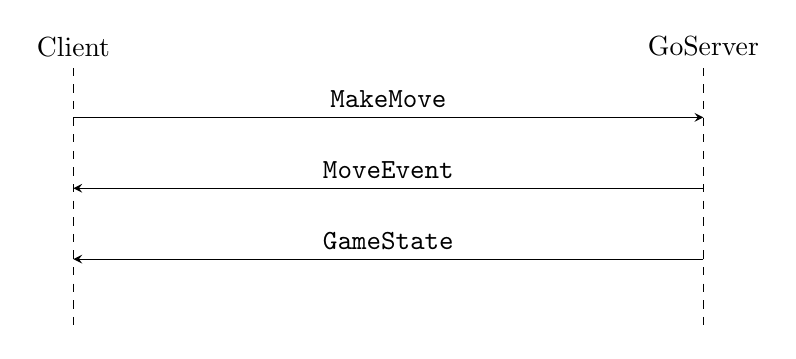
\begin{tikzpicture}[x=1cm,y=0.9cm,>=stealth]
\node (client) at (0,0) {Client};
\node (server) at (8,0) {GoServer};
\draw[dashed] (0,-.3) -- (0,-4);
\draw[dashed] (8,-.3) -- (8,-4);
\draw[->] (0,-1) -- node[above] {\texttt{MakeMove}} (8,-1);
\draw[->] (8,-2) -- node[above] {\texttt{MoveEvent}} (0,-2);
\draw[->] (8,-3) -- node[above] {\texttt{GameState}} (0,-3);
\end{tikzpicture}
\EndAccSupp{}

\caption{Observed successful turn, generated from the actual protocol test
trace, not an independently invented example. Prompt: actually play a game
between two users. Question: did this exchange follow the grammar?
Source: \texttt{evidence/playable-v1/protocol.json}. Reducer: grammar acceptance
plus exact cause/prior checks. Unit: events; boundary: one HTTP turn.}
\end{figure}

\section*{Failure and security boundaries}
R1--R6 in the working contract link to controls and negative tests in
\file{evidence/playable-v1/traceability.json}. Illegal actions, wrong seats,
missing credentials, duplicate submissions and stale revisions cannot change
the requested position. Failed persistence does not publish an uncommitted
action. Snapshots store token hashes, never plaintext seat tokens. Restart
replays and compares every saved position before accepting a room.

Host validation rejects DNS rebinding; Origin validation rejects cross-origin
mutations. Strict UTF-8 JSON rejects duplicate/unknown fields, excess nesting
and oversized bodies. The CLI rejects escaping or symlinked runtime paths.
Boards are at most 19 by 19, there are at most six colors and 512 turns,
local analysis holds at most 2,048 nodes, and storage holds at most 32 rooms
and 64 exports. A GIF contains at most 200 actions; export memory is serialized.
The intended scope is a trusted local operator, not an Internet-facing service.

No screenshot is claimed until the real browser produces it. GIF export
replays selected actions through Go rules, verifies them, then encodes actual
GIF bytes; it never accepts arbitrary filesystem paths. Errors are surfaced
with their failing operation. There is no automatic paid repair/retry loop.
Both PDFs are compiled in scratch directories and promoted only after both
variants succeed; full compiler output is retained on failure.

\section*{Verification and limits}
The differential suite compares every intermediate board, loss ledger,
turn and score in 40 seeded games (2,240 transitions). Go race tests cover
independent seats, simultaneous submissions, deadline Passes, rejected input,
persistence failure and restart. Real HTTP scenarios for all six tasks round-trip
through official protoc-generated bindings and the Lean-derived grammars;
reversed and truncated traces are rejected. Browser traces are checked too.

The browser suite exercises MCTS, keyboard play, sibling variations, selected
GIF download, two isolated seats completing a game, reload recovery and all
121 accessible grid labels. The screenshot on the next page is a real capture.
\file{board-labels.txt} and \file{browser.json} retain its labels and selected
state. These finite checks do not establish general grammar recognition,
checker correctness, strategic competence, network fault tolerance or a formal
Go/JavaScript refinement proof. Those remain explicit follow-up work.

\clearpage
\section*{Captured running application}
\begin{center}
\BeginAccSupp{method=escape,ActualText={Actual running four-player Go application. An eleven by eleven board is shown with the selected recorded position, loss and score tables, signed capture matrix controls, history navigation, MCTS settings, two-player room controls, and verified GIF export. The complete selected state and all 121 cell labels are preserved beside this screenshot.}}
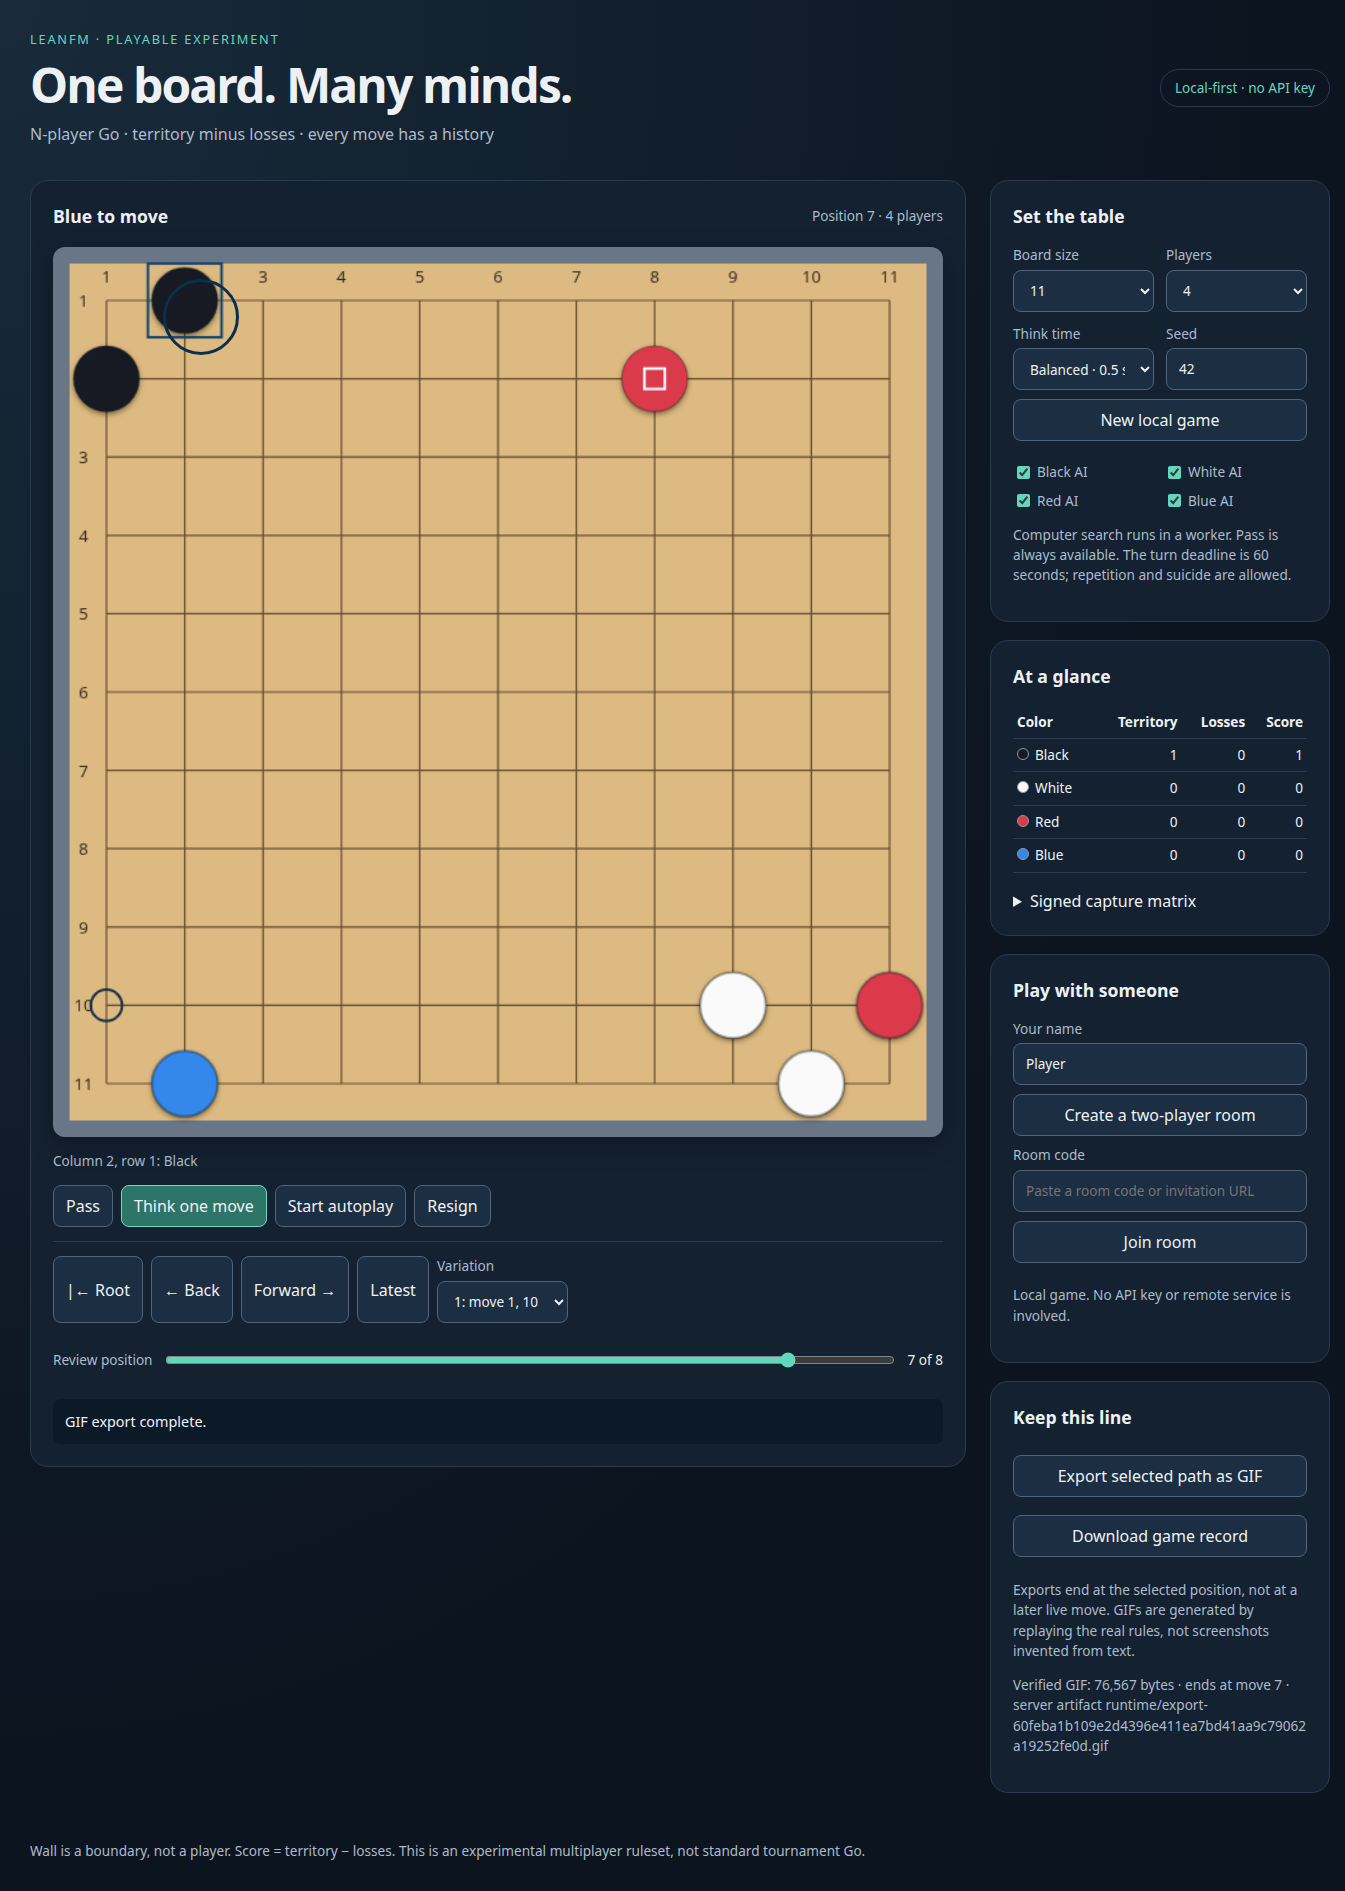
\includegraphics[width=\textwidth,height=0.79\textheight,keepaspectratio]{../evidence/playable-v1/board.png}
\EndAccSupp{}
\end{center}
Prompt: produce a working n-player Go application. Question: does the actual
served UI expose the required controls and selected state? Source: the real
headless browser DOM and canvas. Reducer: capture the selected position after
MCTS, keyboard play and history review. Unit: pixels and labeled cells;
boundary: one browser viewport. This static PDF is not an animation; the real
animation is \file{evidence/playable-v1/selected-line.gif}.
\end{document}
